\documentclass{article}
\usepackage{graphicx}
\usepackage{hyperref}
\usepackage{color}
\usepackage{marginnote}
\usepackage{mathtools}
\usepackage{amsmath}
\usepackage{empheq}
\usepackage{listings}

\newcommand{\hilight}[1]{\colorbox{yellow}{#1}}
\newcommand{\boxedeq}[2]{\begin{empheq}[box={\fboxsep=6pt\fbox}]{align}\label{#1}#2\end{empheq}}

\begin{document}

\title{Discretization of an RC Lowpass Filter}
\author{
	Ross Bencina \\
	\texttt{\url{http://www.rossbencina.com}}\\
	\texttt{rossb@audiomulch.com}
}

\date{\today\footnote{An earlier version appeared as a Google document in July 2014. The current version is archived at \url{https://github.com/RossBencina/dsp-notes}. }}
	
\maketitle

\section{Introduction}

This note derives a digital version of an
analog RC lowpass filter\footnote{\url{https://en.wikipedia.org/wiki/RC_circuit#Series_circuit}}
 using nodal analysis and trapezoidal integration.
It follows the method applied by Andrew Simper in his recent technical notes.\footnote{See Simper's
\href{http://www.cytomic.com/files/dsp/OnePoleLinearLowPass.pdf}{worked example of a one pole lowpass filter} and his other technical papers located at
\url{http://www.cytomic.com/technical-papers}.}
The aim is to lay out the mathematical steps that underpin the method.

Some knowledge of calculus and a little familiarity with linear circuits is assumed (e.g. application of Ohm's Law and Kirchoff's Laws to form nodal equations). Familiarity with digital IIR filters is also assumed (i.e. the idea of a digital filter with state variables and a state update procedure that computes an output sample from an input sample at each time step).

\section{The circuit}

The analog RC lowpass circuit is shown in Figure \ref{fig:RC-lowpass-circuit}.

\begin{figure}[here]
	\centering
	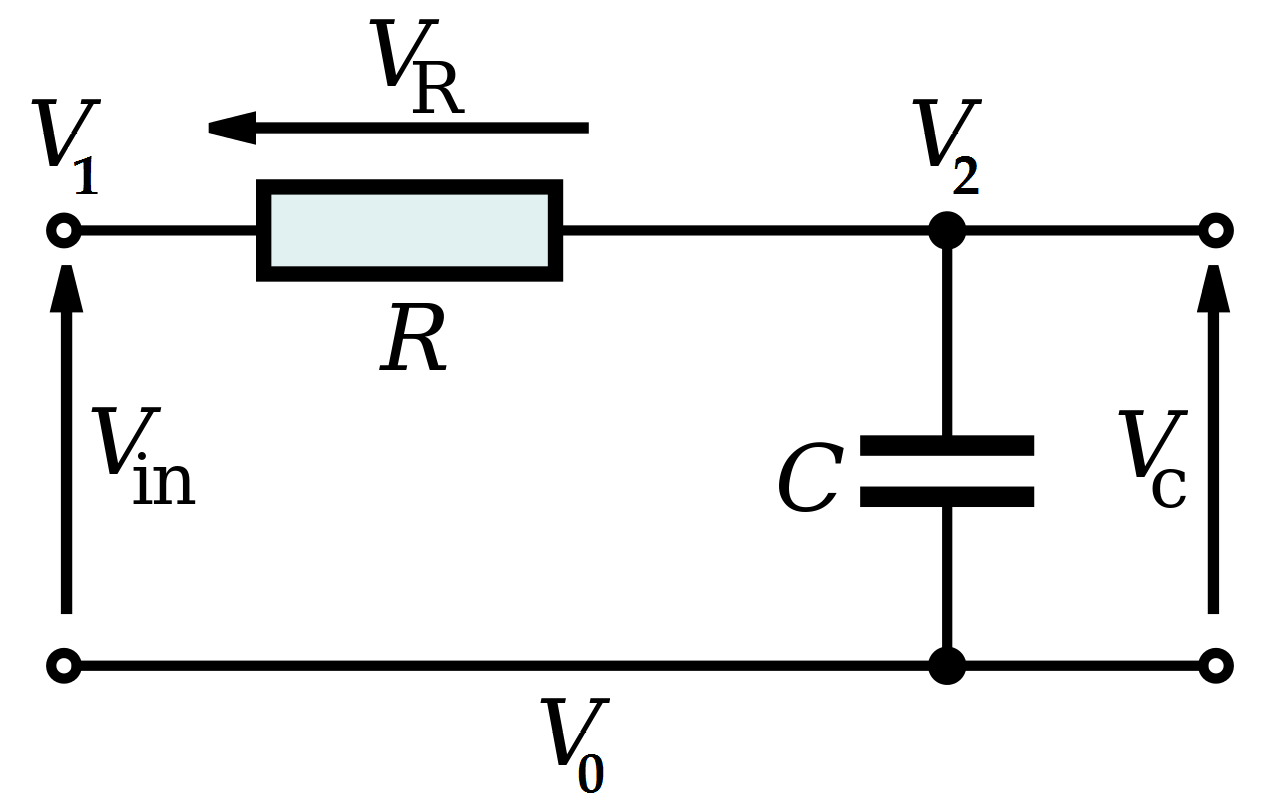
\includegraphics[width=0.5\textwidth]{images/1280px-RC_Series_Filter.png}
	\caption{Analog RC lowpass circuit. 
		Image source: {\href{https://en.wikipedia.org/wiki/File:RC_Series_Filter_(with_V&I_Labels).svg}{Wikipedia}}}
	\label{fig:RC-lowpass-circuit}
\end{figure}

$R$ is the resistance of the resistor.
$C$ is the capacitance of the capacitor.

Our goal is to create a discrete time digital implementation of this circuit.
We want a program that takes $V_{in}$ at each time step and gives us $V_{C}$.
The process of deriving the program involves solving equations for
the circuit using Ohm's Law and Kirchoff's laws. This process is called nodal analysis.\footnote{\url{http://en.wikipedia.org/wiki/Nodal_analysis}}


\section{Voltages across the components}

We assume that electron current flows in the direction of the arrows.\footnote{For our method to succeed, the direction of the arrows doesn't matter so long as they are kept consistent for the whole calculation. See for example \href{https://www.physicsforums.com/threads/node-voltage-analysis.246884/}{this discussion at physicsforums.com}.}
Applying the formula ($V_{highest} - V_{lowest}$) for the votage across a component yeilds the following expressions for the voltages across the resistor and capacitor:

\begin{equation}
V_R = V_{in} - V_C
\end{equation}

\begin{equation}
V_C = V_C - V_0
\end{equation}


\section{Current flow for each component}

We need to know the (effective\footnote{Depending on your point of view, current may not flow ``through''
	capacitors. In our model we're going to assume
	\href{https://www.youtube.com/watch?v=ppWBwZS4e7A}{current flows
		through capacitors} and call it $I_C$.}) current flow through each component.

Recall Ohm's Law for a general resistor:

\boxedeq{}{
	I=\frac{V}{R}
}

This gives us the current through the resistor:

\begin{equation}
\label{eqn:I_R1}
I_R = \frac{1}{R}(V_{in} - V_C)
\end{equation}


The equivalent law for capacitors is:\footnote{\url{https://en.wikipedia.org/wiki/Capacitor#Current.E2.80.93voltage_relation}}

\boxedeq{}{
	I=C\frac{\mathrm{d}V}{\mathrm{d}t}
}

So the current in and out of the capacitor is:

\begin{equation}
\label{eqn:I_C1}
I_C = C\frac{\mathrm{d}}{\mathrm{d}t}V_C
\end{equation}


\section{Not forming a differential equation for the circuit}

Kirchoff's current law (KCL)\footnote{\url{https://en.wikipedia.org/wiki/Kirchhoff's_circuit_laws}}
tells us that the sum of currents into a node
equals the sum of currents out of the node. For node $V_{C}$ this yields

\begin{equation}
I_R = I_C
\end{equation}

Substituting the expressions above for $I_R$ (\ref{eqn:I_R1}) and $I_C$ (\ref{eqn:I_C1}):

\begin{equation}
\frac{1}{R}(V_{in} - V_C) = C\frac{\mathrm{d}}{\mathrm{d}t}V_C
\label{eqn:nodal-equation}
\end{equation}

Our goal is to solve equation \ref{eqn:nodal-equation} for $V_C$ (the circuit output) given $V_{in}$ (the
circuit input) at each time step. Note that we are not going to try
to solve the above differential equation. Instead we discretize
(approximate) the capacitor using a linear approximation and then
expand the KCL equations using the discretized expressions for $I_C$.

\section{Aside: current-voltage relation for a capacitor}

This section is a bit of an aside. We're going to compute a result
that's needed in the next section. It relates capacitor voltage and
current. If you're happy to take the relation as given you can skip this
section. In summary, we will show that equation \ref{eqn:I_C1}:

\begin{equation}
\notag
I_C = C\frac{\mathrm{d}}{\mathrm{d}t}V_C
\end{equation}

implies:

\begin{equation}
\notag
	V_C(t) = \frac{1}{C}\int_{t_0}^{t} \! I_C(\tau) \, \mathrm{d}\tau + V_C(t_0)
\end{equation}

This is a well known relation that expresses voltage across a capacitor
at time $t$ as the sum of the voltage at an earlier time $t_0$, plus an
integration of $I_C$ (current) over the time range $t_0$ to $t$. In the
next section we'll use the relation to construct a discrete time
time-step update equation for the voltage across a capacitor.

To derive the current voltage relation, recall equation \ref{eqn:I_C1}
for current flow in and out of a capacitor:

\begin{align}
\notag
I_C &= C\frac{\mathrm{d}}{\mathrm{d}t}V_C, &\text{(equation \ref{eqn:I_C1})}
\intertext{
rearranging and making time an explicit parameter \tau:
}
\notag
\frac{\mathrm{d}}{\mathrm{d}t}V_C(\tau) &= \frac{1}{C}I_C(\tau) &\hspace{.25\textwidth}
\\
\intertext{
Integrating both sides from $t_0$ to $t$:\footnote{
		See: \url{http://www.site.uottawa.ca/mathasatool/01unit/12topic/focus/voltage_current/p09.htm}
	}
}
\notag
\int_{t_0}^{t} \! \frac{\mathrm{d}}{\mathrm{d}t}V_C(\tau) \, \mathrm{d}\tau
&=
\frac{1}{C}\int_{t_0}^{t} \! I_C(\tau) \, \mathrm{d}\tau
\\
\notag
\left[V_C(\tau)\right]_{t_0}^{t}
&=
\frac{1}{C}\int_{t_0}^{t} \! I_C(\tau) \, \mathrm{d}\tau
\\
\notag
V_C(t) - V_C(t_0)
&=
\frac{1}{C}\int_{t_0}^{t} \! I_C(\tau) \, \mathrm{d}\tau
\\
\label{eqn:V_C_t}
V_C(t)
&=
V_C(t_0) + \frac{1}{C}\int_{t_0}^{t} \! I_C(\tau) \, \mathrm{d}\tau
\end{align}


Notice that given two times $t_0$ and $t$, 
equation \ref{eqn:V_C_t} gives us a way to compute $V_C(t)$ as a function of
$V_C(T_0)$ and a definite integral over $I_C$ from time $t_0$ to
time $t$.


\section{Discretizing a capacitor using the trapezoidal rule}

In the previous section we derived a general time-domain relation (equation \ref{eqn:V_C_t}) for
the capacitor current and voltage in terms of voltage at times
$t_0$ and $t$, and a definite integral of the current from $t_0$ to $t$.
We're going to use the general relation to derive a time-step update
rule (difference equations) for our uniformly sampled (digital) system.
The update rule takes us from the previous time step to the current time
step.

Let $sr$ be the sampling rate in samples per second.

Let $T$ be the sampling period: $T = 1/sr$

Let $t$ be the time of the current time step

Take $t_0$ to be the time of the previous time step, that is $t_0 = t - T$

Discretizing the current/voltage relation for time $t$, first substitute
$t$ and $T$ into the current/voltage relation (\ref{eqn:V_C_t}) from the previous section:

\begin{equation}
\begin{aligned}
V_C(t) &= V_C(t_0) + \frac{1}{C}\int_{t_0}^{t} \! I_C(\tau) \, \mathrm{d}\tau &\hspace{.25\textwidth} &\text{(from equation \ref{eqn:V_C_t})}\\
\label{eqn:V_C_t_a}
       &= V_C(t-T) + \frac{1}{C}\int_{t_0}^{t} \! I_C(\tau) \, \mathrm{d}\tau &&\text{($t_0 = t - T$)}
\end{aligned}
\end{equation}

Now the key step, we apply the trapezoidal rule to discretize the integral.

\begin{align}
\intertext{
	The trapezoidal rule states:\footnote{
		\href{https://en.wikipedia.org/wiki/Trapezoidal_rule}{Trapeziodal rule} (also \href{http://www.mathwords.com/t/trapezoid_rule.htm}{see here}):
	}
}
\label{eqn:trap-rule}
\int_a^b \! f(x) \, mathrm{d}x &\approx (b-a)\frac{(f(a) + f(b))}{2} \\
\intertext{
	We will approximate the following integral:
}
\frac{1}{C}\int_{t_0}^{t} \! I_C(\tau) \, \mathrm{d}\tau &\approx ? \\
\intertext{
	Applying the following substitutions to the trapazoidal rule (\ref{eqn:trap-rule}):
}
f(x)&: I_C(x) \\
a&: (t-T), \\
b&: (t), \\
(b-a) &= t-(t-T) = t-t+T \\
\implies (b-a) &: T\\
\intertext{
	yeilds:
}
\frac{1}{C}\int_{t_0}^{t} \! I_C(\tau) \, \mathrm{d}\tau &\approx \frac{T}{2C} (I_C(t-T) + I_C(t))
\intertext{
	Substituting this approximation into equation \ref{eqn:V_C_t_a} gives an expression for $V_C(t)$ in terms of voltages and currents at the current and previous time steps:
}
\label{eqn:trap-V_C}
V_C(t) &\approx V_C(t-T) + \frac{T}{2C} (I_C(t-T) + I_C(t))
\end {align}

The trapezoidal rule is an approximation, but we will treat equation \ref{eqn:trap-V_C} as an equivalent expression for $V_C$ from here on.

Let's switch our notation to the discrete time domain and to something
more closely resembling computer code.
Take $n$ as the current time step and $n-1$ as the previous time step.
We'll also explicitly notate multiplication using $*$ from now on.
Switch notation as follows:

\begin{align*}
V_C(t) &\to vc[n] \\
V_C(t-T) &\to vc[n-1] \\
I_C(t) &\to ic[n] \\
I_C(t-T) &\to ic[n-1] \\
\end{align*}

Rewriting the trapezoidally integrated equation for $V_C$ (\ref{eqn:trap-V_C}):

\begin{equation}
\label{eqn:trap-V_C-discrete}
vc[n] = vc[n-1] + T/(2C) * ( ic[n-1] + ic[n] )
\end{equation}

Later, when applying KCL we will want an expression for $ic[n]$. So,
	solving equation \ref{eqn:trap-V_C-discrete} for $ic[n]$:

\begin{equation}
vc[n] - vc[n-1] = T/(2C) * ic[n-1] + T/(2C) *  ic[n]
\end{equation}
\begin{equation}
vc[n] - vc[n-1] - T/(2C) * ic[n-1] = T/(2C) * ic[n]
\end{equation}
\begin{equation}
ic[n] = T/(2C) * (vc[n] - vc[n-1]) - ic[n-1]
\end{equation}

Letting $gc = T/(2C)$ gives:

\begin{equation}
ic[n] = gc * vc[n] + (- gc vc[n-1] - ic[n-1])
\end{equation}

Following a convention used by QUCS using ``iceq'':\footnote{
	See e.g. \href{http://qucs.sourceforge.net/tech/node26.html#SECTION00731000000000000000}{equations 6.60 and 6.63 in the QUCS documentation}}

Let

\begin{eqnarray} \begin{array}{l}
iceq[n-1] = - gc * vc[n-1] - ic[n-1]\\
ic[n] = gc * vc[n] + iceq[n-1].
\end{array} \end{eqnarray}

Or equivalently:

\begin{eqnarray} \begin{array}{l}
ic[n] = gc * vc[n] + iceq[n-1]\\
iceq[n] = - gc vc[n] - ic[n].
\end{array} \end{eqnarray}

We can further simplify $iceq$ by substituting for $ic[n]$

\begin{eqnarray} \begin{array}{l}
iceq[n] = - gc*vc[n] - ic[n]\\
iceq[n] = - gc*vc[n] - (gc * vc[n] + iceq[n-1])\\
iceq[n] = -2*gc*vc[n] - iceq[n-1].
\end{array} \end{eqnarray}


\section{Solving the KCL equation(s) using the linear equivalent capacitor current}

Remember the differential equation that we didn't solve earlier? We're
going to solve the equivalent linear equation. Instead of 
$I_C = C\frac{\mathrm{d}}{\mathrm{d}t}V_C$
we'll be using the linear approximation ($ic[n]$) that we just derived.

Recall,

\begin{equation}
gc = 2C/T
\end{equation}

\begin{equation}
\begin{aligned}
		   I_R &= (1/R) (V_{in} - V_C)	 	&\text{(current through the resistor)} \\
\to	     ir[n] &= (1/R) (vin[n] - vc[n])    \hspace{.1\textwidth}& \\
\\
	     ic[n] &= gc * vc[n] + iceq[n-1]    &\text{(current ``through'' the capacitor)}
\end{aligned}
\end{equation}

Equating current in and current out at our node of interest:

\begin{equation}
\begin{aligned}
                   I_R &= I_C	 	&\text{(currents in and out of a node are equal)} \\
                 ir[n] &= ic[n]	\hspace{.1\textwidth}& \\
(1/R) (vin[n] - vc[n]) &= gc * vc[n] + iceq[n-1]
\end{aligned}
\end{equation}

\textit{
(In general we would have a set of simultaneous equations to
	solve, one equation for each node. However, in this case we have only
	one node.)
}


Now the final step. Given our input $vin[n]$ we want to compute $vc[n]$

Solving the previous equation for $vc[n]$:

\begin{equation}
\begin{aligned}
     (1/R) (vin[n] - vc[n]) &= gc * vc[n] + iceq[n-1] \\
(1/R) * vin[n] - (1/R *) vc[n] - gc * vc[n] - iceq[n-1] &= 0 \\
(1/R) * vin[n] - iceq[n-1] 	&= (1/R) * vc[n] + gc * vc[n] \\
vin[n] - R * iceq[n-1] 		&= vc[n] + R * gc * vc[n]			&\text{(multiply by R)} \\
                            &= vc[n] * (1 + R*gc) \\
                  vc[n] 	&= (vin[n] - R * iceq[n-1]) / (1 + R*gc)
\end{aligned}
\end{equation}

So our final equations in pseudo-code form are:

\begin{lstlisting}
init:
    T = 1 / sr
    gc = T/(2C)
    iceq = 0

step:
    vc[n] = (vin[n] - R * iceq[n-1]) / (1 + R*gc)
    iceq[n] = (- 2*gc*vc[n] - iceq[n-1]).
\end{lstlisting}

or, letting gr = 1/R

\begin{lstlisting}
step:
    vc[n] = (gr * vin[n] - iceq[n-1]) / (gr + gc)
    iceq[n] = (- 2*gc*vc[n] - iceq[n-1])
\end{lstlisting}

Or equivalently:

\begin{lstlisting}
step:
    vc[n] = (gr * vin[n] + iceq[n-1]) / (gr + gc)
    iceq[n] = 2*gc*vc[n] - iceq[n-1]
\end{lstlisting}

Andrew Simper suggests setting gc=1, gr=g

\begin{lstlisting}
step:
    vc[n] = (g * vin[n] + iceq[n-1]) / (1 + g)
    iceq[n] = 2*vc[n] - iceq[n-1]
\end{lstlisting}


\section{Acknowledgements}

The method described here is an interpretation of
{\href{http://www.google.com/url?q=http\%3A\%2F\%2Fwww.cytomic.com\%2Ffiles\%2Fdsp\%2FOnePoleLinearLowPass.pdf\&sa=D\&sntz=1\&usg=AFQjCNFFyauZI4XmAtL0x26dzTBQzY-GXQ}{Andrew
		Simper's worked example here}}{, and in
}{\href{http://www.google.com/url?q=http\%3A\%2F\%2Fwww.cytomic.com\%2Ftechnical-papers\&sa=D\&sntz=1\&usg=AFQjCNGwKW2UyEgVuFPUWhxGkyl0Cq9VLA}{his
	related papers here}}{. Thanks to Andrew and other members of the
\#musicdsp IRC channel for their very kind assistance in guiding me
through this.

\end{document}